% Compiles with IEEEtran (e.g. on Overleaf). If IEEEtran.cls is not installed,
% it falls back to a two-column article with IEEE-like margins and headings.
\IfFileExists{IEEEtran.cls}{%
  \documentclass[conference]{IEEEtran}
  \newif\ifieee\ieeetrue
}{%
  \documentclass[10pt,twocolumn,letterpaper]{article}
  \newif\ifieee\ieeefalse
}
\ifieee\else
  \usepackage[top=0.75in,bottom=1in,left=0.625in,right=0.625in,columnsep=0.25in]{geometry}
  \usepackage{mathptmx}
  \usepackage[T1]{fontenc}
  \usepackage{titlesec}
  \renewcommand{\thesection}{\Roman{section}}
  \renewcommand{\thesubsection}{\Alph{subsection}}
  \titleformat{\section}{\centering\normalsize\scshape}{\thesection.}{0.5em}{}
  \titleformat{\subsection}{\normalsize\itshape}{\thesubsection.}{0.5em}{}
  \titlespacing*{\section}{0pt}{8pt}{4pt}
  \titlespacing*{\subsection}{0pt}{6pt}{3pt}
  \usepackage[font=footnotesize,labelsep=period]{caption}
  \newcommand{\IEEEauthorblockN}[1]{{\large #1}\\}
  \newcommand{\IEEEauthorblockA}[1]{\normalsize\itshape\begin{tabular}{@{}c@{}}#1\end{tabular}}
  \newenvironment{IEEEkeywords}{\par\noindent\textbf{\textit{Index Terms}---}\itshape}{\par}
  \renewenvironment{abstract}{\par\noindent\textbf{\textit{Abstract}---}\bfseries}{\par\medskip}
  \pagestyle{plain}
\fi
\usepackage{amsmath}
\usepackage{graphicx}
\usepackage{booktabs}
\usepackage{cite}
\usepackage{url}
\graphicspath{{../figures/}}

\begin{document}

\title{Climate or Design? Mission-Profile Thermal Cycling of Electric Two-Wheeler Motor Controllers in Five Cities}

\author{\IEEEauthorblockN{Syeda Tehreem Gillani}
\IEEEauthorblockA{Department of Computer Science, FAST National University of Computer and Emerging Sciences, Karachi, Pakistan}}

\maketitle

\begin{abstract}
Electric two-wheelers are sold mostly in hot countries, and their motor
controllers use low-cost discrete MOSFETs. This paper asks how much a hot
climate adds to the thermal cycling of such a controller, and how that
compares with design and use choices. A 2~kW, 72~V scooter is driven on the
WMTC test cycle with the official road load of UN GTR No.~2. Losses of an
inverter built from IRFB4115 MOSFETs are taken from the datasheet, and a
heatsink model turns them into junction temperature, second by second,
for a full year of 2025 NASA POWER weather in Karachi, Delhi, Jakarta,
Lagos and Madrid, for a commuter and a delivery rider. Cycles are counted
by rainflow and weighted with a Coffin-Manson-Arrhenius law anchored to the
part's own qualification test. For cycles caused by riding, the hot cities
see 1.1 to 2.6 times the damage of Madrid, and Delhi ranks first under 63 of
72 life-model choices; most of the spread comes from the assumed activation
energy. Design and use factors move the damage far more: a poorly cooled
box multiplies it by about 17, using 12 instead of 18 MOSFETs by about 9.
In absolute terms the cycling damage stays small even in a hard-use case,
so hot-climate problems are more likely to appear as thermal-limit events
(13.5 riding hours a year above an 80~\textdegree C heatsink in Delhi
delivery use) than as solder or bond-wire wear-out.
\end{abstract}

\begin{IEEEkeywords}
electric two-wheeler, motor controller, MOSFET, mission profile, thermal cycling, rainflow, reliability
\end{IEEEkeywords}

\section{Introduction}
Electric scooters and motorcycles are growing fast in South and Southeast
Asia. In Pakistan, for example, about 33{,}000 electric motorbikes were
sold in 2024 and about 57{,}800 in the first seven months of 2025
\cite{profit2025}. The controller of such a vehicle is a three-phase
inverter, usually built from discrete TO-220 MOSFETs on an aluminium case.
It works in heat, in stop-and-go traffic, and often with a passenger or
cargo.

Mission-profile methods, which turn a real use pattern into temperature
swings and then into consumed life, are now a standard reliability tool for
power electronics \cite{wang2013}. They have been applied to PV inverters
in different climates \cite{brito2018} and to SiC inverters for motor
drives, including electric traction \cite{barbagallo2021}. For electric two-wheelers, recent work has looked
at the thermal behaviour of the hub motor \cite{deshmukh2026} and at the
heatsink of the controller in steady and transient runs \cite{tripathi2023},
but we did not find a study that follows the controller's semiconductors
through a year of real weather and compares climates.

One difficulty is that the usual life models (LESIT \cite{held1997}, CIPS08
\cite{bayerer2008}) were fitted for IGBT modules, and in a recent review the
only model fitted on discrete packages comes from TO-247 IGBTs, none from
discrete MOSFETs \cite{wang2025}.
We therefore use the life law only to rank conditions, check how the ranking
depends on the model, and anchor the scale to the qualification test that
the manufacturer published for this exact part \cite{infineonqual}.

The contributions are: (i) an open pipeline in which every input comes from
a named public source (GTR No.~2, the MOSFET datasheet, NASA POWER); (ii) a
comparison of five cities for two kinds of riders; (iii) a ranking of
design and use factors against climate; and (iv) a check of all rankings
over 36 life-model settings.

\section{Models}
\subsection{Vehicle and drive cycle}
The vehicle is a scooter of the type sold in Pakistan: 102~kg dry mass,
2~kW hub motor, 70~km/h top speed, 90/90-10 tyres \cite{garipk}, 72~V
battery \cite{pakwheels}. With the 75~kg driver of GTR No.~2 the mass in
running order is $m_{ref}=177$~kg. The road load is the running resistance
table of GTR No.~2, Annex~3 \cite{gtr2}: for $175<m_{ref}\le185$~kg,
$F=a+bv^2$ with $a=15.8$~N and $b=0.0227$~N/(km/h)$^2$. For rotating parts
we add 7\,\% of the mass: the regulation's estimates of 3\,\% for the front
wheel and 4\,\% for the rear wheel with the parts rotating with it, here the
hub motor. The table was made for
conventional motorcycles and is used here as the official reference.

The speed trace is part~1 of the WMTC (600~s, 4.065~km, up to 60~km/h),
read from the tables of GTR No.~2 \cite{gtr2}. By maximum speed the scooter
falls in the 50--100~km/h band of subclass 1-3, which uses part~1; an
electric vehicle has no engine capacity, so this mapping is our choice.

WMTC asks for up to about 4.1~kW, more than a 2~kW scooter delivers, so the
controller limits the motor to a 100~A peak phase current and 3~kW from the
battery, of which 88\,\% reaches the wheel (assumed values, varied later). The scooter follows the trace as
closely as these limits allow; the RMS speed error is 1.6~km/h. The model
needs 18.7~Wh/km at the wheel. The claimed 120~km range on a 2.52~kWh pack
implies about 21~Wh/km at the battery, which leaves room for motor and
controller losses, so we take the model as plausible.

The motor is a direct-drive PMSM under field-oriented control. Its back-EMF
constant is set so that the phase back-EMF at top speed is 90\,\% of
$V_{dc}/\sqrt3$, giving $k_e=0.40$~V\,s/rad and a peak phase current
$I=T/(1.5k_e)$. There is no regenerative braking in the base case.

\subsection{MOSFET losses}
Each of the six switches has $N$ IRFB4115 devices in parallel, $N=3$ in the
base case (an ``18-MOSFET'' controller). From the datasheet \cite{infineonds}:
$R_{DS(on)}=9.3$~m$\Omega$ typical at 25~\textdegree C with the temperature
curve of its Fig.~4 (read by eye, about $\pm0.05$), $t_r=73$~ns, $t_f=39$~ns, $Q_{rr}=300$--450~nC. With
complementary gating each switch carries on average
$P_{cond}=R_{DS(on)}(T_J)\,(I/N)^2/4$. Switching loss is linear in current
and voltage, $E=\tfrac12 V_{dc}\bar I(t_r+t_f)$ with $\bar I=2I/(\pi N)$,
plus $Q_{rr}V_{dc}$, at 15~kHz. Because a real gate drive is slower than the
datasheet test circuit, the switching times are doubled in the base case.
At 100~A and $T_J=50$~\textdegree C the loss is 4.6~W per device, two
thirds of it conduction.

\subsection{Thermal model}
The datasheet gives $R_{thJC}=0.4$~K/W as a two-element Foster network with
time constants of 5.9 and 0.63~ms, and $R_{thCS}=0.5$~K/W. At 1~s steps the
junction-to-case drop is therefore quasi-static,
$T_J=T_{hs}+P(R_{thJC}+R_{thCS})$. The controller box is one thermal mass,
$C_{hs}\dot T_{hs}=P_{tot}-(T_{hs}-T_{amb})/R_{hs}$, with $C_{hs}=450$~J/K
(about 0.5~kg of aluminium) and $R_{hs}=0.5$~K/W while riding. Both are
assumptions and are varied.

\subsection{Weather and use}
$T_{amb}$ is the hourly 2~m air temperature (MERRA-2 based) from NASA POWER
\cite{nasapower} for 2025 at the five city centres. In earlier work on the
Karachi files we found that POWER's ``LST'' is the nominal zone of the
longitude, not civil time \cite{gillani2026}; we apply the same rule to all
cities, with summer time for Madrid. Table~\ref{tab:base} gives the
climates: Delhi has the hottest hours (956 above 35~\textdegree C, maximum
45.9~\textdegree C), Jakarta and Lagos are warm but never reach
35~\textdegree C, and Madrid has a cool mean but 212 hours above
35~\textdegree C.

Two riders are simulated. The commuter rides Monday to Saturday at 08:00 and
17:30, each ride three WMTC part~1 cycles (30~min, 12~km). The delivery rider
rides every day, twelve rides from 11:00 to 22:00, each two cycles (20~min,
8~km), about 96~km a day. All 365 days are stepped together, one second at
a time.

\subsection{Cycle counting and damage index}
The junction temperature is reduced to reversals with 0.5~K hysteresis and
counted with the three-point rainflow method of ASTM E1049 \cite{astm1049},
which we implemented and tested against a hand count. Two countings are
compared: per day (all cycles, including the slow swing of the air
temperature between a morning and an evening ride) and per ride (only the
cycles caused by riding, each ride plus 15~min of cooling).

Damage is $D=\sum n_i/N_f(\Delta T_i,T_{m,i})$ with
$N_f=A\,\Delta T^{-n}\exp(E_a/k_BT_m)$. The qualification report of
IRFB4115 lists an intermittent operational life test (MIL-STD-750 method
1037) at $\Delta T=100$~K for 8572 cycles with no failure in 231 parts
\cite{infineonqual}. We set $N_f(100~\text{K})=8572$ with an assumed mean of
75~\textdegree C. This treats a passed test as a failure, so $D$ is
pessimistic; $D=1$ means as much cycling as the whole test, not end of life.
The base model uses $n=5$ from the LESIT model and $E_a=0.617$~eV from a
Coffin-Manson-Arrhenius module model, both as listed in \cite{wang2025}; $n=3$--6, $E_a=0$--0.617~eV and a minimum counted
range of 0, 2 or 5~K give 36 settings. Ratios between cities do not depend
on $A$.

\section{Results}
\subsection{Base case}
The controller runs cool in the base case (Table~\ref{tab:base}). The mean
junction rise over the air while riding is 5.9--6.6~K in every city, and the
hottest junction of the year is 41--58~\textdegree C. The cities differ
in the level the cycles ride on, not in their size. Fig.~\ref{fig:day}
shows the delivery rider on Delhi's hottest day.

\begin{table}[t]
\centering
\caption{Climate and base-case results (delivery rider; damage per year)}
\label{tab:base}
\footnotesize
\setlength{\tabcolsep}{3.5pt}
\begin{tabular}{lrrrrr}
\toprule
 & Karachi & Delhi & Jakarta & Lagos & Madrid\\
\midrule
mean $T_{amb}$ (\textdegree C) & 26.3 & 24.8 & 27.6 & 26.8 & 14.4\\
max $T_{amb}$ (\textdegree C) & 40.4 & 45.9 & 32.0 & 32.2 & 40.6\\
hours $>35$\textdegree C & 173 & 956 & 0 & 0 & 212\\
max $T_J$ (\textdegree C) & 52.5 & 58.2 & 43.4 & 43.7 & 52.6\\
$D$, per-ride count ($10^{-7}$) & 6.9 & 8.2 & 6.3 & 6.0 & 3.7\\
ratio to Madrid & 1.86 & 2.22 & 1.71 & 1.61 & 1.00\\
\bottomrule
\end{tabular}
\end{table}

\begin{figure}[t]
\centering
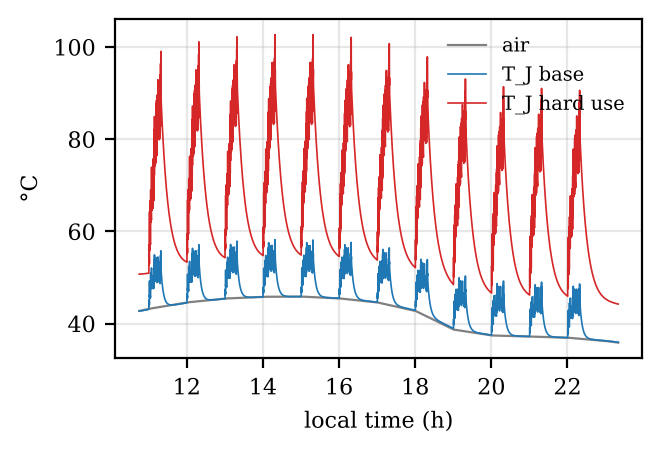
\includegraphics[width=\columnwidth]{f2_day_delhi.png}
\caption{Delivery rider on the hottest day of 2025 in Delhi: air
temperature, junction temperature in the base case, and in the hard-use
case of Section~III-D (whose air is 8~K warmer inside the body).}
\label{fig:day}
\end{figure}

\subsection{How much does the climate matter?}
Counting only the cycles caused by riding (Fig.~\ref{fig:ratio}a), every hot
city sees more damage than Madrid: 1.6 to 2.2 times for the delivery rider
and 2.0 to 2.4 times for the commuter in the base model, and 1.1 to 2.6
times over all 36 settings. Delhi is the most damaged city in 35 of 36
settings for the delivery rider and in 28 of 36 for the commuter (Jakarta
in the others). Most of the effect comes from the activation energy: with
$E_a=0$ the ratios fall to 1.13--1.50, which is what the larger $R_{DS(on)}$
at high temperature and the larger cycles alone give.

The whole-day counting tells a different story for the commuter
(Fig.~\ref{fig:ratio}b): Madrid becomes the most damaged city in 30 of 36
settings. In Madrid 97\,\% of the commuter's damage comes from half cycles,
the dry-climate swing of the air (on average 11.9~K between the coolest
and warmest moment of the riding day, against 2.4~K in Jakarta). Power-cycling laws were fitted
to cycles of seconds to minutes, not to swings of ten hours, so we regard
the per-ride result as the more reliable one and report the other as a
warning: the choice of counting can reverse a climate ranking.

\begin{figure*}[t]
\centering
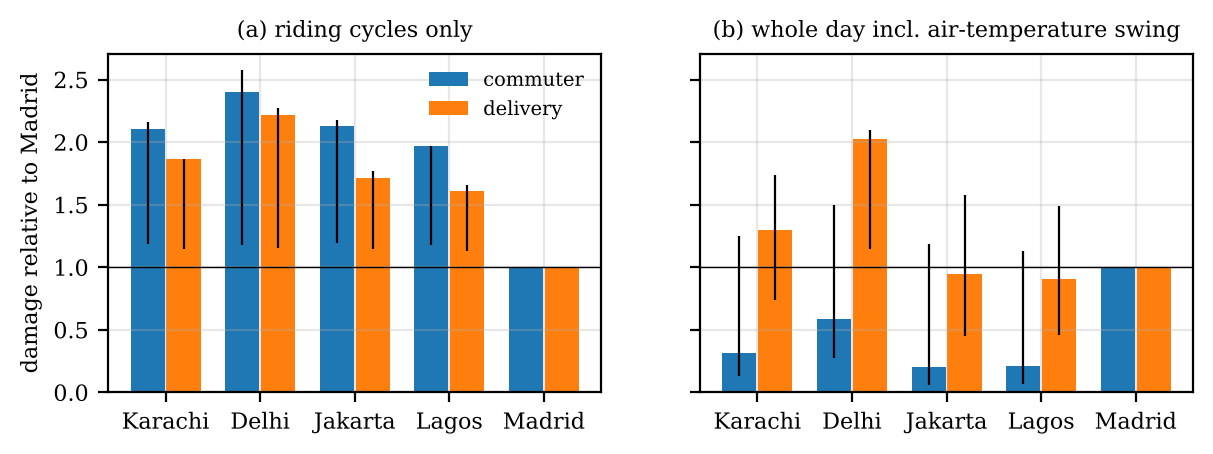
\includegraphics[width=0.85\textwidth]{f3_ratio.png}
\caption{Damage relative to Madrid. Bars: base life model ($n=5$,
$E_a=0.617$~eV, ranges $\ge2$~K). Lines: range over all 36 life-model
settings. (a) cycles counted per ride; (b) counted per day, including the
slow swing of the air temperature.}
\label{fig:ratio}
\end{figure*}

\subsection{Design and use against climate}
Fig.~\ref{fig:factors} changes one factor at a time for the delivery rider
in Delhi (per-day counting). A box with no airflow ($R_{hs}=1.5$~K/W)
multiplies the damage by 17.0, a 12-MOSFET controller by 9.2, a controller
tuned for 150~A and 4.5~kW by 5.8, a gate drive four times slower than the
datasheet by 3.9, and a passenger or 75~kg of cargo by 2.8. Eight kelvin of
extra heat inside the body, which is a climate-like change, gives 2.1,
regenerative braking 1.8 and the worst-case $R_{DS(on)}$ 1.6. The same order holds in Karachi and Madrid.
Every design and use factor we tried is of the same size as the climate
effect or larger.

\begin{figure}[t]
\centering
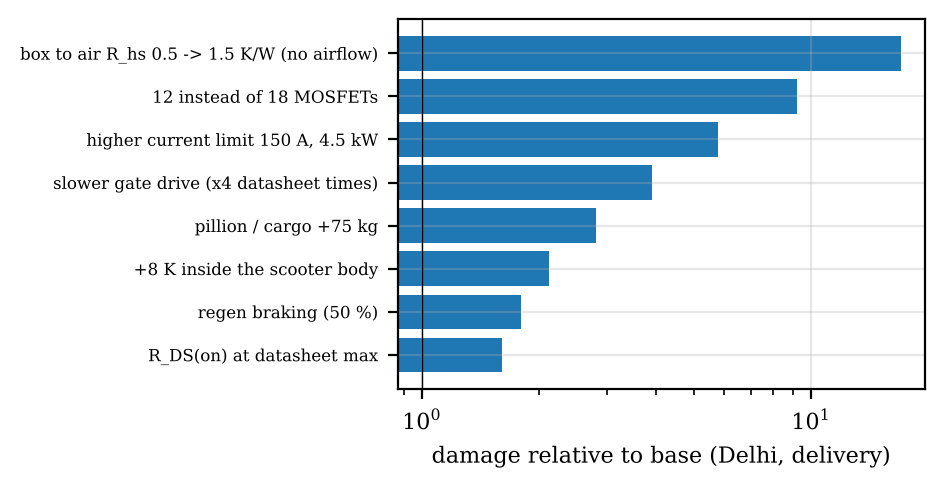
\includegraphics[width=\columnwidth]{f4_factors.png}
\caption{One factor at a time, delivery rider in Delhi: damage relative to
the base case (log scale).}
\label{fig:factors}
\end{figure}

\subsection{Hard use}
The hard-use case combines a box with no airflow, 12 MOSFETs, 8~K of body
heat and 75~kg of extra load. The junction then reaches 84--106~\textdegree C
and the largest cycle of the year for the delivery rider in Delhi
reaches 63~K (Fig.~\ref{fig:day}). With delivery use the
heatsink is above 80~\textdegree C for 13.5 riding hours a year in Delhi,
1.0 in Madrid, 0.5 in Karachi and never in Jakarta or Lagos. A controller
that protects itself by reducing power near such a temperature would do so
mostly in Delhi, almost all of it in April, May and June. The damage index
rises about 2200 times for the delivery rider in Delhi (between about 1000
and 7000 times across all cases) but stays at $3.5\times10^{-3}$ per year
($2.3\times10^{-2}$ with $n=3$), that is, at most about 2.3\,\% of the
qualification test's cycling each year even with the pessimistic anchor.

\section{Discussion and Limitations}
Within this model, climate changes the thermal-cycling damage of a scooter
controller by a factor of about two, while cooling and the number of MOSFETs
change it by about an order of magnitude. Because the
absolute damage is small, a hot climate is more likely to show up as
reduced power at the thermal limit, or through mechanisms not modelled here,
than as bond-wire or solder fatigue of the MOSFETs. For manufacturers
selling into hot cities, the cooling path of the box and the device count
are the levers that matter, and summer peaks in places like Delhi are the
cases to check.

The study has clear limits. Nothing is validated against measurements of a
real controller; the box thermal resistance and capacity, the controller
limits, the body-heat offset and the use profiles are assumptions, which
is why they are varied. The road load table was written for conventional
motorcycles, WMTC has no hills, and real city traffic in these countries may
be harsher than WMTC. Losses are averaged over an electrical period, which
misses the slow current pulsation at walking speed. The air temperature is
not the temperature inside the scooter in the sun. The life law is
extrapolated from 100~K to cycles of a few kelvin and was fitted for
modules, so the absolute damage index is an indicator, not a lifetime.
Only one year of weather is used.

\section{Conclusion}
An open, fully sourced mission-profile model of an electric two-wheeler
controller shows that hot cities add roughly 1.1--2.6 times the thermal
cycling of Madrid, with Delhi worst in 63 of 72 settings, while design and use
factors change it by up to 16--21 times. The result also depends on how the
cycles are counted, which future studies should state. Measuring the case
temperature of a real controller in summer delivery use would be the next
step, and would let the assumed thermal parameters be replaced by data.

\section*{Acknowledgment}
AI-based coding assistance was used for parts of the simulation software and
the first draft of the text. The modelling choices, results and text were
checked by the author.

\section*{Code and Data}
\url{https://github.com/tehreem-gillani/e2w-controller-wearout}. Weather:
NASA POWER hourly 2025. Drive cycle and road load: UN GTR No.~2. Device data:
Infineon IRFB4115PbF datasheet and product qualification report.

\begin{thebibliography}{99}
\footnotesize
\bibitem{profit2025} ``Sales of EV motorbikes surge despite infrastructural challenges,'' \emph{Profit by Pakistan Today}, Aug. 2025. [Online]. Available: \url{https://profit.pakistantoday.com.pk/?p=209085}
\bibitem{wang2013} H. Wang, M. Liserre, and F. Blaabjerg, ``Toward reliable power electronics: Challenges, design tools, and opportunities,'' \emph{IEEE Ind. Electron. Mag.}, vol. 7, no. 2, pp. 17--26, 2013.
\bibitem{brito2018} E. M. S. Brito, A. F. Cupertino, P. D. Reigosa, Y. Yang, V. F. Mendes, and H. A. Pereira, ``Impact of meteorological variations on the lifetime of grid-connected PV inverters,'' \emph{Microelectronics Reliability}, 2018, doi: 10.1016/j.microrel.2018.07.066.
\bibitem{barbagallo2021} C. Barbagallo, S. A. Rizzo, G. Scelba, G. Scarcella, and M. Cacciato, ``On the lifetime estimation of SiC power MOSFETs for motor drive applications,'' \emph{Electronics}, vol. 10, no. 3, art. 324, 2021, doi: 10.3390/electronics10030324.
\bibitem{deshmukh2026} S. Deshmukh, N. Lokhande, and S. Yeolekar, ``Predictive temperature control of electric two wheeler hub motor using gradient aware neural regulation with degradation tracking and fault tolerant multi condition torque adaptation,'' \emph{Scientific Reports}, vol. 16, 2026, doi: 10.1038/s41598-026-37505-y.
\bibitem{tripathi2023} K. Tripathi, A. Ghosh, A. Mangal, M. Sreejeth, and S. Indu, ``Thermal study of MOSFET heat sinks for motor controller in neighbourhood electric vehicles,'' \emph{Int. J. Electric and Hybrid Vehicles}, vol. 15, no. 3, pp. 256--271, 2023.
\bibitem{held1997} M. Held, P. Jacob, G. Nicoletti, \emph{et al.}, ``Fast power cycling test of IGBT modules in traction application,'' in \emph{Proc. 2nd Int. Conf. Power Electronics and Drive Systems (PEDS)}, 1997, vol. 1, pp. 425--430.
\bibitem{bayerer2008} R. Bayerer, T. Herrmann, J. Lutz, \emph{et al.}, ``Model for power cycling lifetime of IGBT modules: Various factors influencing lifetime,'' in \emph{Proc. 5th Int. Conf. Integrated Power Electronics Systems (CIPS)}, Nuremberg, Germany, 2008, pp. 1--6.
\bibitem{wang2025} W. Wang, B. Ren, M. Pan, Y. Zhou, E. Deng, and Y. Huang, ``State-of-the-art of power cycling lifetime models for power electronics,'' \emph{Chinese J. Electrical Engineering}, vol. 11, no. 4, pp. 60--74, 2025, doi: 10.23919/CJEE.2024.000095.
\bibitem{infineonqual} Infineon Technologies, ``Product qualification report: IRFB4115, Trench MV,'' Rev. 1.0.
\bibitem{garipk} ``Evee C1 Air specifications,'' gari.pk. [Online]. Available: \url{https://www.gari.pk/bikes/evee/c1-air}, accessed Oct. 2026.
\bibitem{pakwheels} ``Evee C1 Air price in Pakistan, pictures and specs,'' PakWheels. [Online]. Available: \url{https://www.pakwheels.com/bikes/evee/c1-air--2/}, accessed Oct. 2026.
\bibitem{gtr2} UNECE, ``Global technical regulation No. 2: Measurement procedure for two-wheeled motorcycles equipped with a positive or compression ignition engine with regard to the emission of gaseous pollutants, CO2 emissions and fuel consumption,'' ECE/TRANS/180/Add.2, 2005.
\bibitem{infineonds} Infineon Technologies, ``IRFB4115PbF datasheet,'' Rev. 2.1, Aug. 2026.
\bibitem{nasapower} NASA Langley Research Center, ``Prediction of Worldwide Energy Resources (POWER) project, hourly API,'' [Online]. Available: \url{https://power.larc.nasa.gov}, accessed Oct. 2026.
\bibitem{gillani2026} S. T. Gillani, ``Look-ahead battery reserve for rooftop PV under scheduled load-shedding: A perfect-foresight benchmark study for Karachi,'' code and results, GitHub repository, 2026. [Online]. Available: \url{https://github.com/tehreem-gillani/pv-battery-ems-karachi}
\bibitem{astm1049} ASTM International, ``Standard practices for cycle counting in fatigue analysis,'' ASTM E1049-85.
\end{thebibliography}

\end{document}
